\documentclass{article}
\usepackage[utf8]{inputenc} %кодировка
\usepackage[T2A]{fontenc}
\usepackage[english,russian]{babel} %русификатор 
\usepackage{mathtools} %библиотека матеши
\usepackage[left=1cm,right=1cm,top=2cm,bottom=2cm,bindingoffset=0cm]{geometry} %изменение отступов на листе
\usepackage{amsmath}
\usepackage{graphicx} %библиотека для графики и картинок
\graphicspath{}
\DeclareGraphicsExtensions{.pdf,.png,.jpg}
\usepackage{subcaption}
\usepackage{pgfplots}
\usepackage{float}
\usepackage{hyperref}


\begin{document}
% НАЧАЛО ТИТУЛЬНОГО ЛИСТА
\begin{center}
    \Large
    Федеральное государственное автономное \\
    образовательное учреждение высшего образования \\ 
    «Научно-образовательная корпорация ИТМО»\\
    \vspace{0.5cm}
    \large
    Факультет программной инженерии и компьютерной техники \\
    Направление подготовки 09.03.04 Программная инженерия \\
    \vspace{1cm}
    \Large
    \textbf{Отчёт по лабораторной работе №1} \\
        По дисциплине «Бизнес логика программных систем» ( семестр 6)\\
    \large
    \vspace{8cm}

    \begin{minipage}{.33\textwidth}
    \end{minipage}
    \hfill
    \begin{minipage}{.4\textwidth}
    
        \textbf{Студент}: \vspace{.1cm} \\
        \ Дениченко Александр\\
        \ Разинкин Александр\\
        \textbf{Практик}:  \\
        \ Бобрусь Александр
    \end{minipage}
    \vfill
Санкт-Петербург\\ 2025 г.
\end{center}
\pagestyle{empty}
% КОНЕЦ ТИТУЛЬНОГО ЛИСТА 
\newpage
\pagestyle{plain}

\section*{Данные}
\begin{center}
    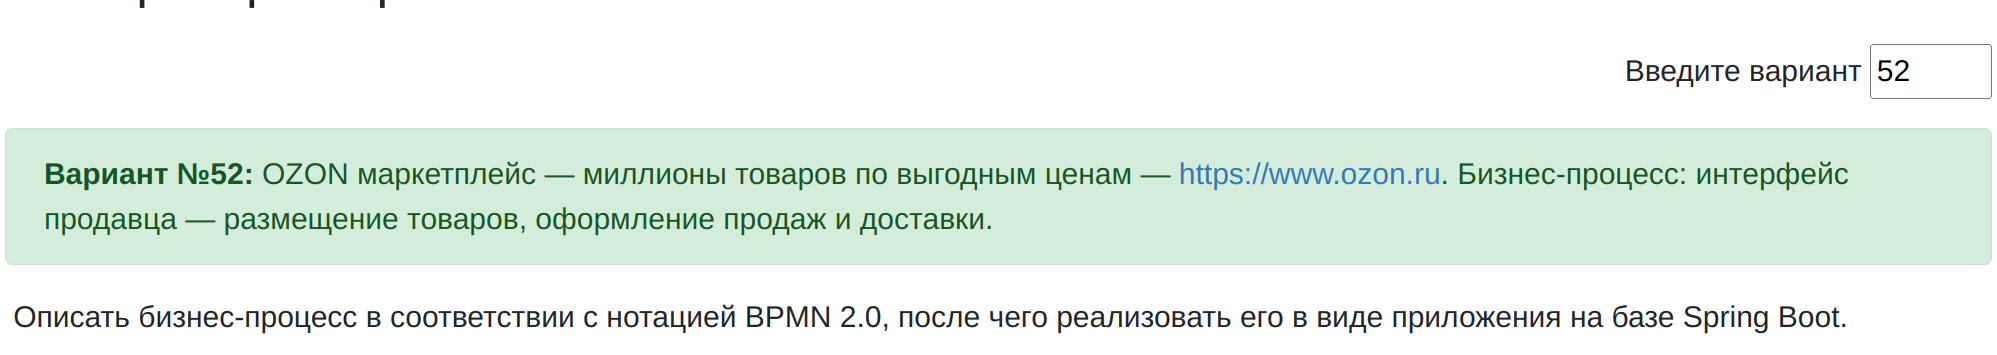
\includegraphics[width=.9\textwidth]{lab}
\end{center}

\section*{BPMN}
\begin{center}
    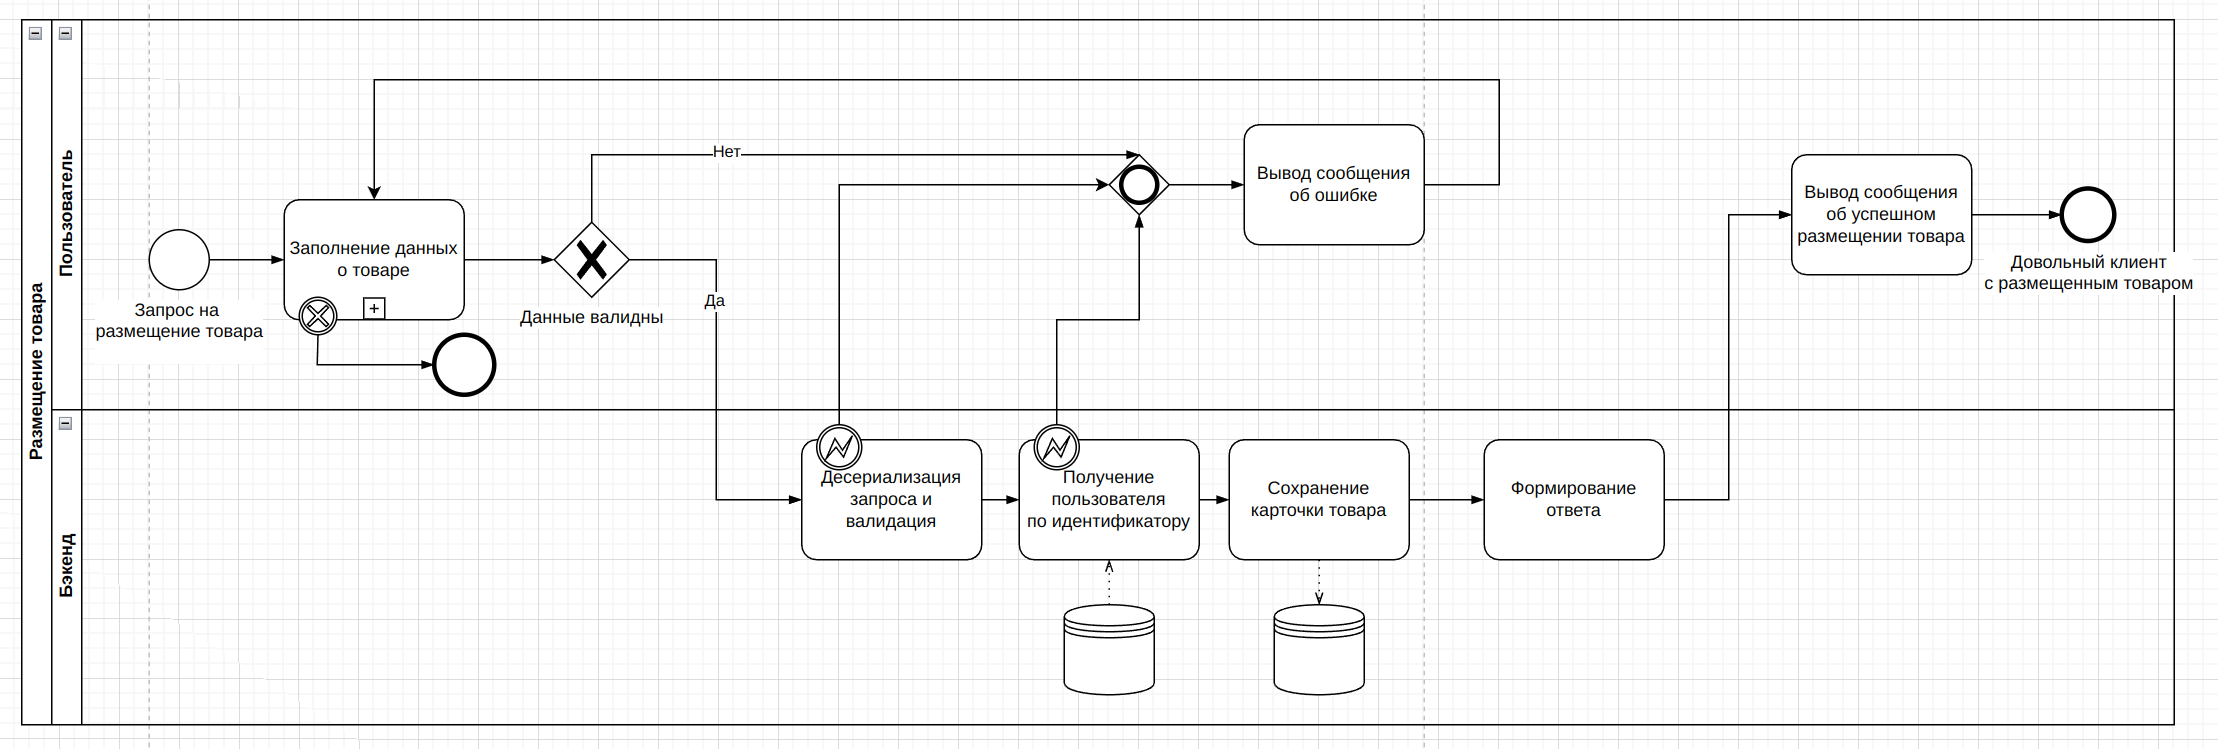
\includegraphics[width=.9\textwidth]{bpmn1}
\end{center}
\begin{center}
    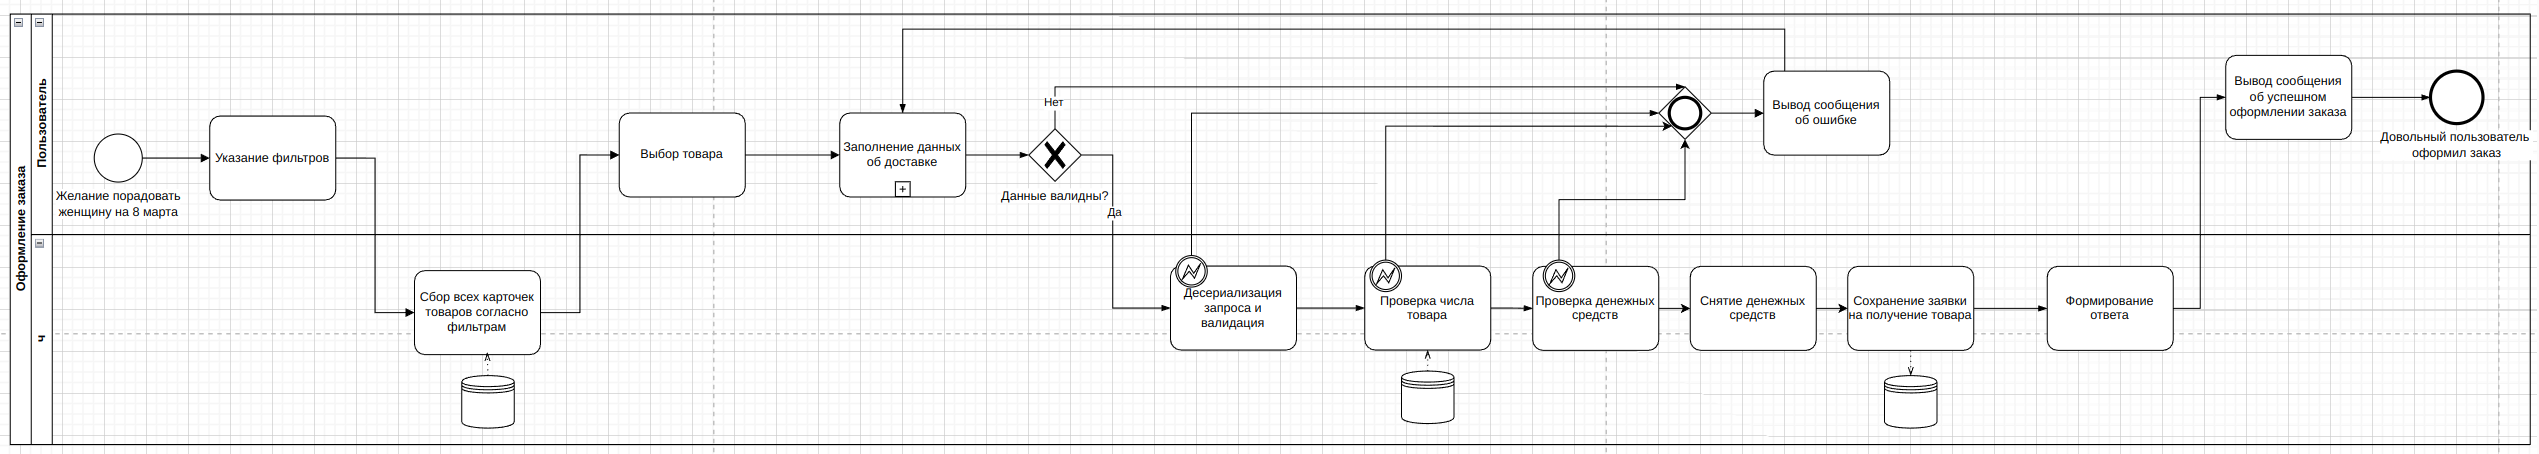
\includegraphics[width=.9\textwidth]{bpmn2.png}
\end{center}
\begin{center}
    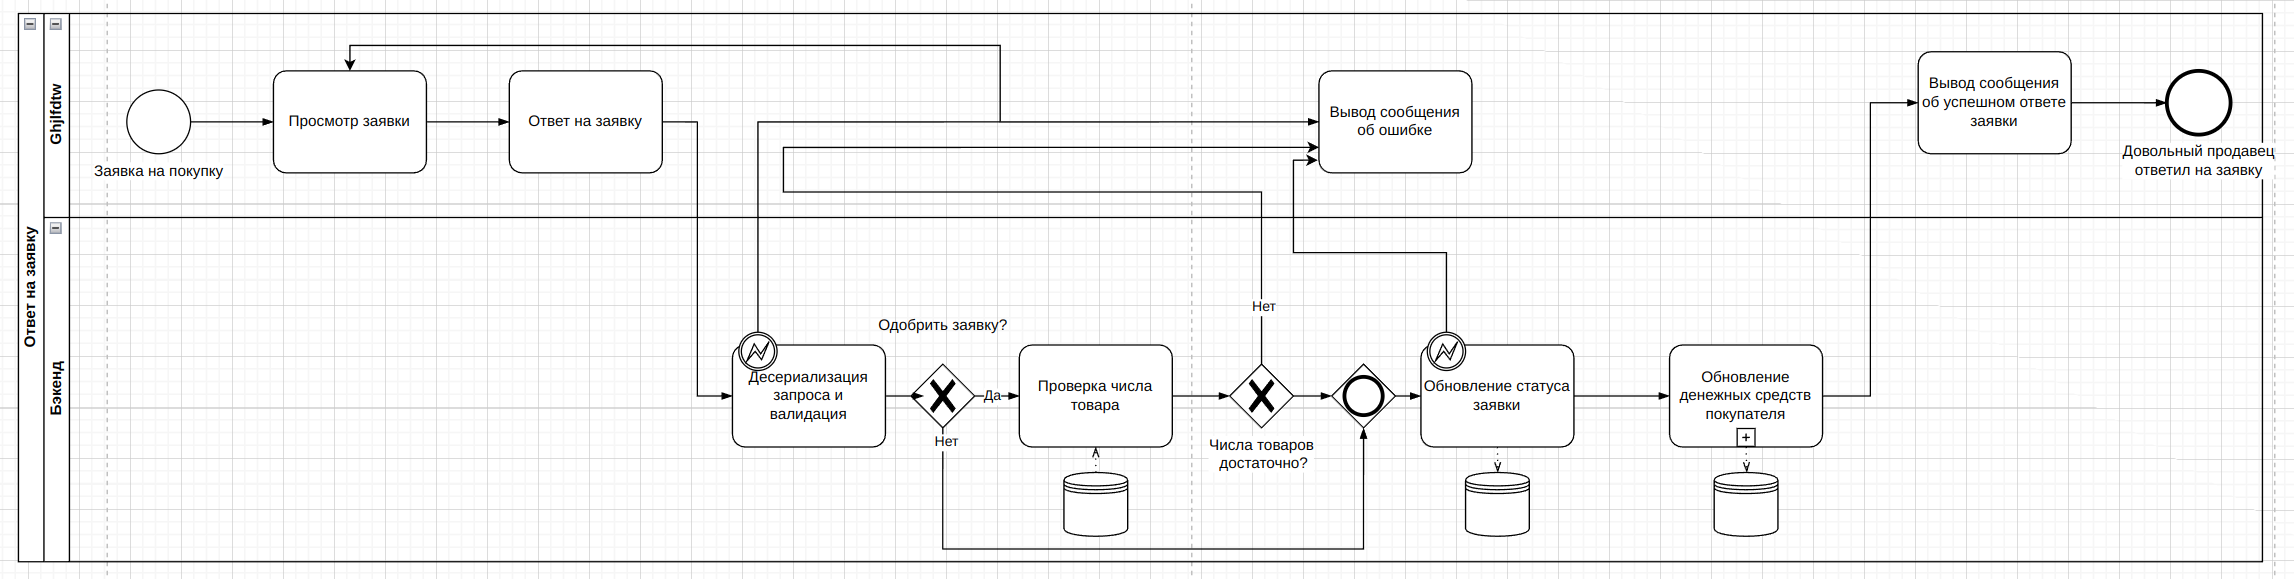
\includegraphics[width=.9\textwidth]{bpmn3.png}
\end{center}

\section*{Спецификация REST API}
\begin{center}
    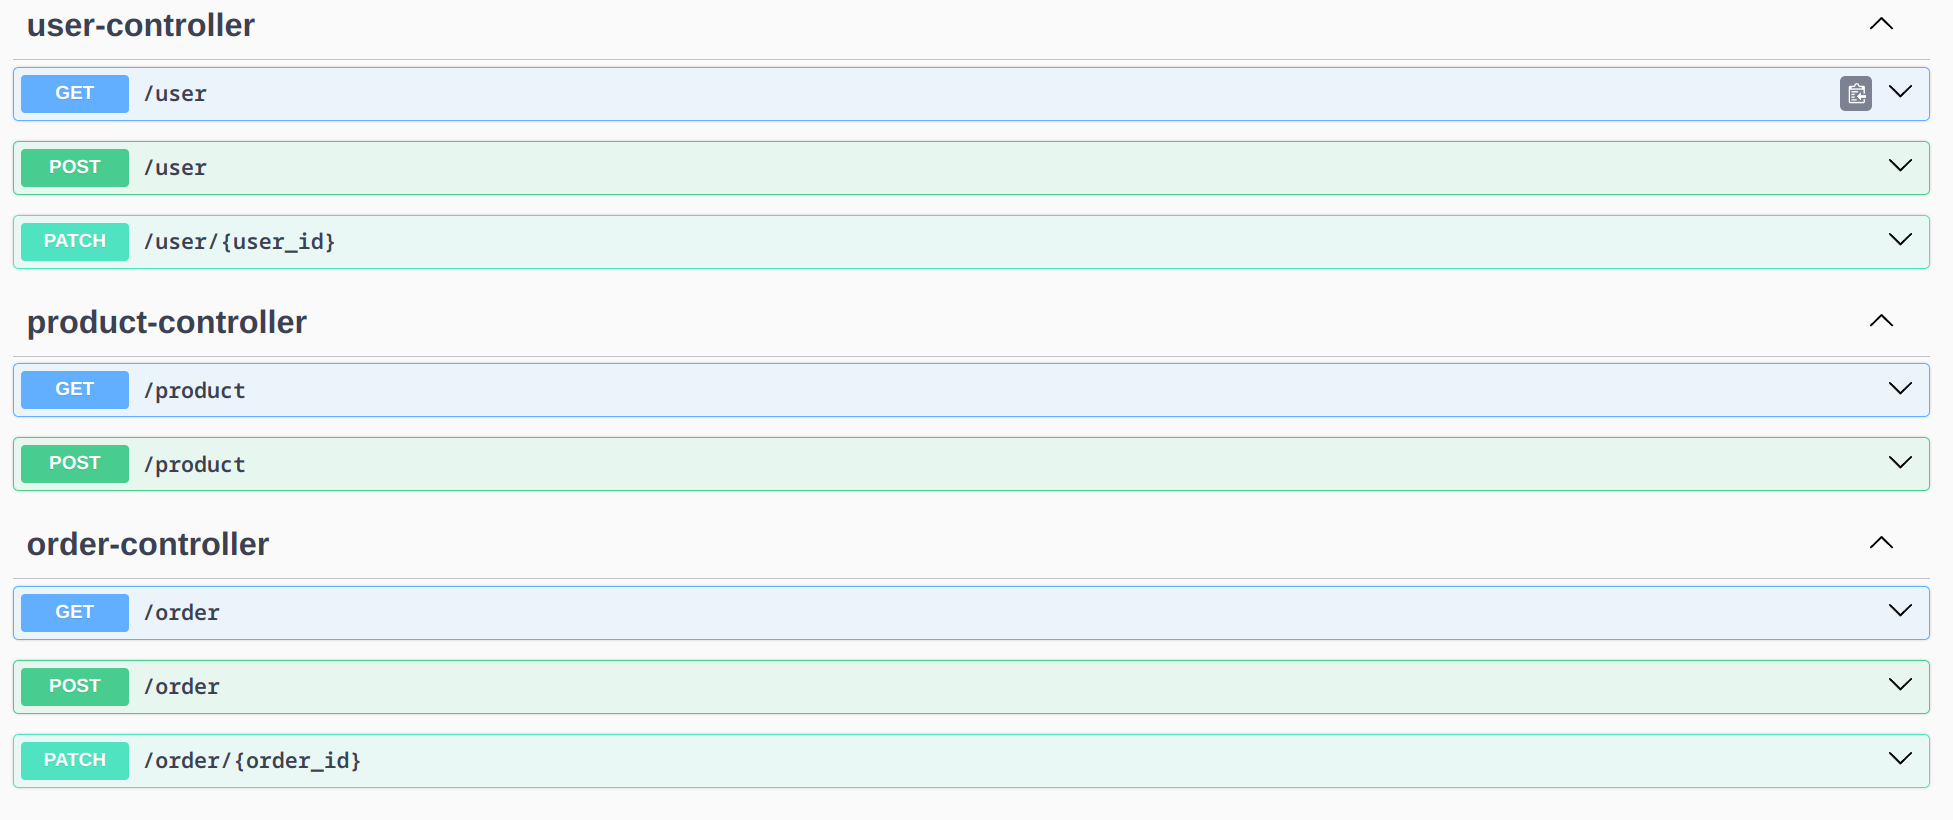
\includegraphics[width=.9\textwidth]{rest1.png}
\end{center}


\url{https://github.com/DecafMangoITMO/blps_lab1}

\section*{Вывод}
Спроектирована диаграмма бизнес процессов при помощи BPMN. Разработан базовый функционал по диаграмме на базе Spring Boot.
Написан сприкт для postman для тестирования функционала. Сделано документирование REST API для всех публичных интерфейсов разработанного приложения.

\end{document}
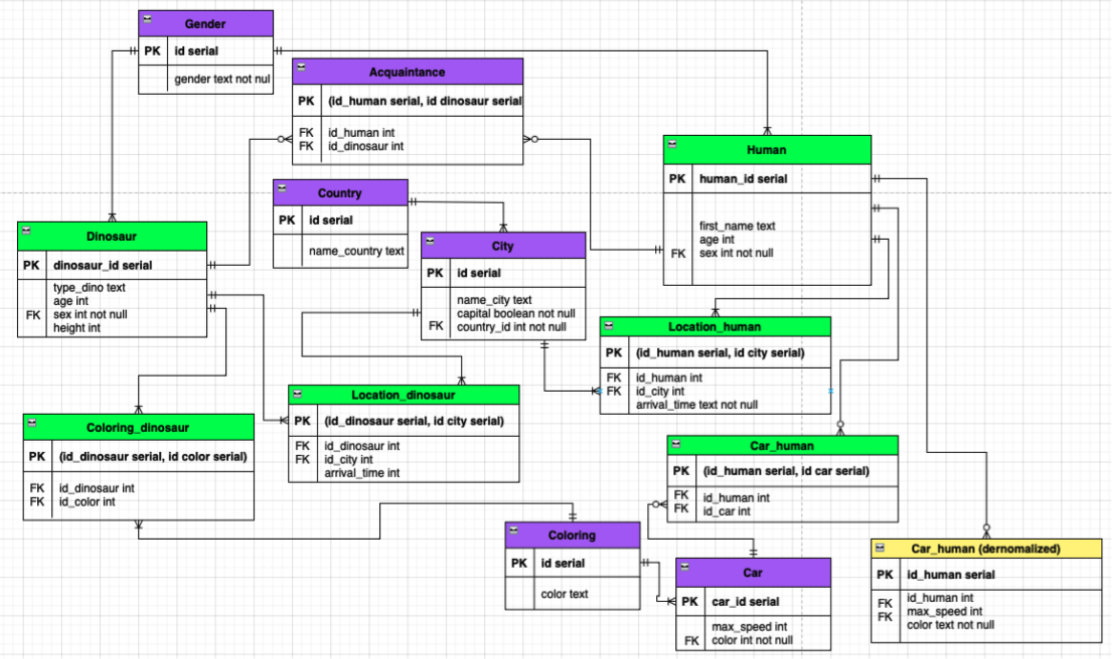
\includegraphics[width=.9\textwidth]{123}